\let\negmedspace\undefined
\let\negthickspace\undefined
\documentclass[journal]{IEEEtran}
\usepackage[a5paper, margin=10mm, onecolumn]{geometry}
%\usepackage{lmodern} % Ensure lmodern is loaded for pdflatex
\usepackage{tfrupee} % Include tfrupee package

\setlength{\headheight}{1cm} % Set the height of the header box
\setlength{\headsep}{0mm}     % Set the distance between the header box and the top of the text

\usepackage{gvv-book}
\usepackage{gvv}
\usepackage{cite}
\usepackage{amsmath,amssymb,amsfonts,amsthm}
\usepackage{algorithmic}
\usepackage{graphicx}
\usepackage{textcomp}
\usepackage{xcolor}
\usepackage{txfonts}
\usepackage{listings}
\usepackage{enumitem}
\usepackage{mathtools}
\usepackage{gensymb}
\usepackage{comment}
\usepackage[breaklinks=true]{hyperref}
\usepackage{tkz-euclide} 
\usepackage{listings}
% \usepackage{gvv}                                        
\def\inputGnumericTable{}                                 
\usepackage[latin1]{inputenc}                                
\usepackage{color}                                            
\usepackage{array}                                            
\usepackage{longtable}                                       
\usepackage{calc}                                             
\usepackage{multirow}                                         
\usepackage{hhline}                                           
\usepackage{ifthen}                                           
\usepackage{lscape}
\usepackage{circuitikz}


\author{EE25BTECH11041-Naman Kumar }
\graphicspath{./figs/}

\begin{document}
\begin{center}
    \huge{2.8.23}\\
    \large{EE25BTECH11041 - Naman Kumar}
\end{center}
Question:\\
If a variable line in two adjacent positions has directions cosines l, m, n and $l+\delta l, m+\delta m, n +\delta n$, show that the small angle $\delta\theta$ between the two positions is given by
\begin{center}
    $\delta\theta^2=(\delta l)^2+(\delta m)^2+(\delta n)^2$
\end{center}
\solution \\
We know about direction cosine of any vector,
\begin{align}
    l^2+m^2+n^2=1 \label{1}
\end{align}
and angle between two vectors
\begin{align}
    \cos{\theta}=\frac{\Vec{A}^T\Vec{B}}{\lVert\Vec{A}\rVert\lVert\Vec{B}\rVert} \label{2}
\end{align}
We also know expansion of $\cos{\delta x}$ ($\delta x$ represents very small x)
\begin{align}
    \cos{\delta x}= 1-\frac{x^2}{2!}+\frac{x^4}{4!}.... \label{3}
\end{align}
Given Two direction cosine
\begin{align}
    l,m,n \text{ and } l+\delta l,m+\delta m,n+\delta n
\end{align}
Using $\eqref{1}$ for both direction cosines
\begin{align}
    l^2+m^2+n^2=1
\end{align}
and
\begin{align}
    (l+\delta l)^2+(m+\delta m)^2+(n+\delta n)^2=1\\
    l^2+m^2+n^2+(\delta l)^2+(\delta m)^2+(\delta n)^2+2(l\delta l+m\delta m+n\delta n)=1
\end{align}
from $\eqref{1}$
\begin{align}
    1+(\delta l)^2+(\delta m)^2+(\delta n)^2+2(l\delta l+m\delta m+n\delta n)=1\\
    (\delta l)^2+(\delta m)^2+(\delta n)^2=-2(l\delta l+m\delta m+n\delta n) \label{9}
\end{align}
Using equation $\eqref{2}$
\begin{align}
    \cos{\theta}=\frac{\begin{pmatrix}l\\m\\n\end{pmatrix}^T \begin{pmatrix}l+\delta l\\m+\delta m\\n+\delta n\end{pmatrix}^T}{1\times 1}\\
    \cos{\theta}=l(l+\delta l)+m(m+\delta m)+n(n+\delta n)\\
    \cos{\theta}=l^2+m^2+n^2+l\delta l+m\delta m+n\delta n\\
\end{align}
using equation $\eqref{1}$ $\eqref{2}$ and $\eqref{9}$
\begin{align}
    1-\frac{\delta\theta^2}{2!}=1+\frac{1}{-2}(\delta l)^2+(\delta m)^2+(\delta n)^2
\end{align}
Where $\delta\theta$ represents very small $\theta$
\begin{align}
\delta\theta^2=(\delta l)^2+(\delta m)^2+(\delta n)^2
\end{align}
Hence Proved
\begin{figure}[H]
    \centering
    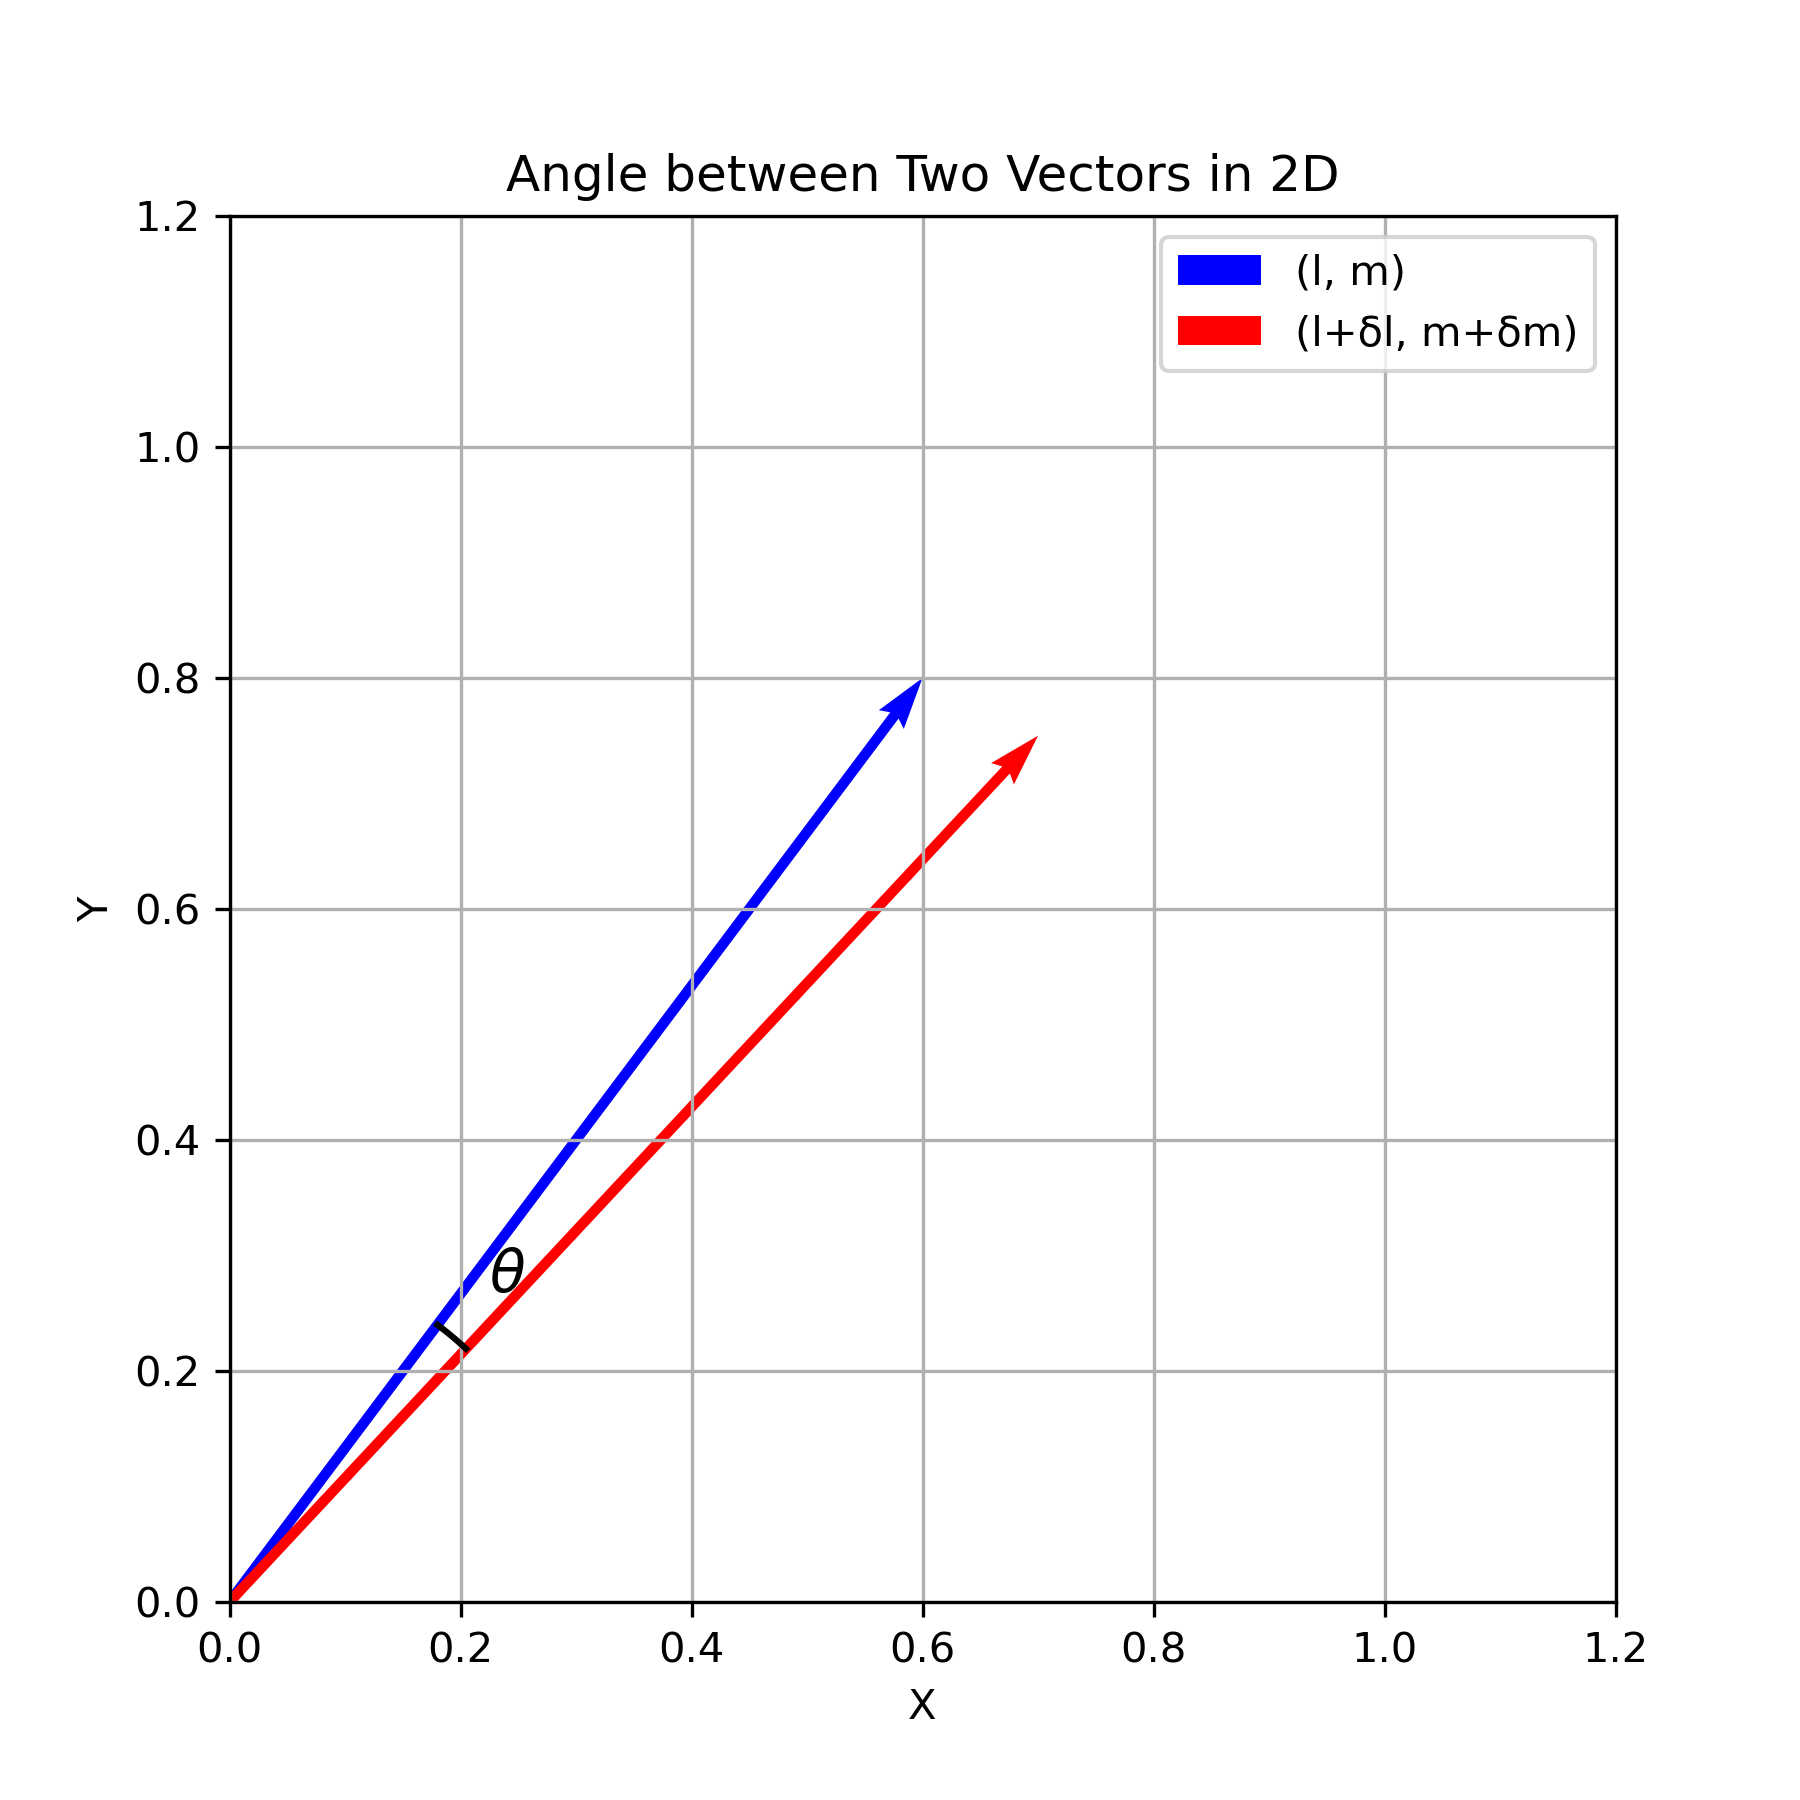
\includegraphics[width=\columnwidth]{figs/vectors.png}
    \caption{Caption}
    \label{fig:placeholder}
\end{figure}
\end{document}
